%% 第二章--chapter2.tex
\chapter{代码说明}\label{chap:CodeIntro}
本章将简单说明编译文档所需代码,
推荐将本文档与源代码结合起来阅读。


\section{摘要和关键词}\label{sec:abstract}
    \emph{摘要}部分的源文件位于\texttt{chapter/abstract.tex},在相应位置输入文本即可。

    下面是中英文摘要分为两页的一个最小示例:

    \begin{lstlisting}[caption=双页摘要\LaTeX{} 代码最小示例]
\begin{abstract}
    \addcontentsline{toc}{chapter}{摘要}        % ``摘要''编入目录
	在此键入中文摘要。
	\vspace{1em}
    % 这里需要空行
	\heiti{关键词:}{关键词}\quad {关键词} \quad  {关键词}
\end{abstract}
\begin{abstracten}
    \addcontentsline{toc}{chapter}{ABSTRACT}    % ``ABSTRACT''编入目录
	Input English abstract here.
	\vspace{1em}
    % Skip a line necessary here.
	\textbf{{KEYWORDS:}{KEYWORD}\quad {KEYWORD}\quad {KEYWORD}}
\end{abstracten}        
    \end{lstlisting}

    本文档的中、英文摘要分成了两页,
    因为若将300字的中文摘要、1500字符的英文摘要及其关键字排版在一页中,行间距会比较狭窄。
    若您仍需要排版在同一页,请改用\texttt{abstractsame和abstractsameen}环境。

    同时,为防止摘要部分溢出一页,
    宏包中对中文标题、``摘要''二字、英文标题和``ABSTRACT''
    所在行的\texttt{beforeskip}和\texttt{afterskip}设为0,
    而内容与双页摘要相同。
    若有需要,您可使用\texttt{$\backslash$setlength\{$\backslash$baselineskip\}\{\ \}}命令及参数控制行距,并可在相应位置插入\texttt{$\backslash$vspace\{ \}}命令及参数或修改宏包文件以控制垂直间距。


\section{目录}\label{sec:content}
    在\texttt{buctthesis.tex}中以

    \begin{lstlisting}[firstnumber=38]
\tableofcontents
    \end{lstlisting}
    命令生成\emph{目录}。默认
    编入\emph{诚信申明、中英文摘要、前言、章、结论、符号说明、参考文献、附录}、节、小节,
    不编入\emph{封面、目录}、小小节(subsubsection)及各列表环境、方程、图片与表格,
    且将``第1章''设置为第1页。
    
    若不需要需要将\emph{摘要}编入目录,
    请将\texttt{abstract.tex}中

	\begin{lstlisting}
\addcontentsline{toc}{chapter}{摘要}
    \end{lstlisting}
    
	\begin{lstlisting}
\addcontentsline{toc}{chapter}{ABSTRACT}
	\end{lstlisting}
    两处代码注释或删除;
    
    若需要将\emph{前言}从目录中删除,参见\ref{subsec:fwtoc}。
    
    
\section{前言}\label{sec:foreword}
	前言部分的源代码位于\texttt{chapter/foreword.tex},在相应位置输入文本即可。
    \subsection{页码设置}\label{subsec:fwpage}
    若需要将\emph{前言}设置为第1页,请将\texttt{buctthesis.tex}文件中

    \begin{lstlisting}[firstnumber=61]
%% 前言--foreword.tex
\begin{foreword}
    \addcontentsline{toc}{chapter}{前言}    % 编入目录
    这里是前言。
    点明毕业论文的论题、学术意义以及其与所阅读文献的关系,简要说明文献收集的目的、重点、时空范围、文献种类、核心刊物等方面的内容。

    关于这一部分的设置请参见第 \ref{sec:foreword} 节。
\end{foreword}


    \end{lstlisting}
    移至正文部分。
    \subsection{编目设置}\label{subsec:fwtoc}
    若要将\emph{前言}编入\emph{目录},
    请在源文件中注释或删除
    \begin{lstlisting}[firstnumber=3]
\addcontentsline{toc}{chapter}{前言}
    \end{lstlisting}

\section{正文}
正文部分各个章节的源文件存放于\texttt{chapter/}文件夹,
在\texttt{buctthesis.tex}正文部分以

\begin{lstlisting}
\include{chapter/filename.tex}
\end{lstlisting}
命令插入各章节。以此命令插入的文件可以不带扩展名
,此时默认扩展名为\texttt{.tex}。

使用\texttt{$\backslash$include}命令会在读入文件前另起一页,
若不希望这样,可以使用
\begin{lstlisting}
\input{chapter/filename.tex}
\end{lstlisting}
此命令相当于纯粹插入文件里的内容。
    \subsection{图片}\label{subsec:fig}
    一般的图片插入使用\texttt{figure}环境:

    \begin{lstlisting}[caption=插入图片,label=code:addfig]
\begin{figure}[H]
    \centering
    \includegraphics[width=0.4\textwidth]{figure/buctlogo.ai}
    \caption{校徽和校名}
    \label{fig:logo}
\end{figure}        
    \end{lstlisting}
    
    就能像这样插入一张图片:
    \begin{figure}[H]
        \centering
        \includegraphics[width=0.4\textwidth]{figure/WholeLogo.ai}
        \caption{校徽和校名}
        \label{fig:WholeLogo}
    \end{figure}
    后文引用:北化的校徽和校名见图\ref{fig:WholeLogo}。

    一般来说图片使用\texttt{$\backslash$centering}命令居中对齐,如果需要如下并排图片,
	    \begin{figure}[H]
        \centering
        \subfigure[这是校名]{
            \label{fig:znname} 
            
\includegraphics[width=4cm]{figure/ZNName.png}}
        \hspace{1cm}
        \subfigure[这是校徽]{
            \label{fig:logo}
            
\includegraphics[scale=0.4]{figure/Logo.pdf}}
        \caption{校名和校徽}
        \label{fig:wholelogo}
    \end{figure}
	可以使用这样的代码:
    
    \begin{lstlisting}[caption=插图并列,label=code:2figs]
\begin{figure}[H]
    \centering                          % 组图整体居中
    \subfigure[这是校名]{               % 第一张插图的标题
        \label{fig:znname}
        
\includegraphics[width=4cm]{figure/ZNName.png}}
    \hspace{1cm}
    \subfigure[这是校徽]{               % 第二张插图的标题
        \label{fig:logo}
        
\includegraphics[scale=0.4]{figure/Logo.pdf}}
    \caption{校名和校徽}                % 组图的标题
    \label{fig:wholelogo}
\end{figure}
    \end{lstlisting}


    在代码\ref{code:addfig}和\ref{code:2figs}展示了三种不同的图片格式和三种不同的方法来控制所插入图片的大小。
    \subsection{公式}\label{subsec:eq}
        公式分为编号和不编号的两类。可以使用\texttt{equation}环境为公式编号,如下所示:
        \begin{lstlisting}
\begin{equation}\label{eq:gougu}
    a^2+b^2=c^2
\end{equation}    
        \end{lstlisting}
        \begin{equation}\label{eq:gougu}
            a^2+b^2=c^2
        \end{equation}
        后文可以这样引用:我在这里引用\ref{eq:gougu}这个式子,或者使用这样的\eqref{eq:gougu}。

        下面这个是不编号的公式:使用\texttt{equation*}环境:
        \begin{equation*}
        x_{1,2}=\frac{{-b \pm \sqrt{{b^2}-4ac}}}{{2a}}.
        \end{equation*}
        行内公式可以用美元符号\texttt{\$ \$},如$f(x)=ax^2+bx+c$.

        对于上述\texttt{equation*}环境中的公式,可以用双美元符号\texttt{\$\$ \quad{}\$\$}或\texttt{$\backslash$[ \quad{}$\backslash$]}。下面是一个例子:
    
    令$f(x)=ax^2+bx+c=0$,则$x^2+\dfrac{b}{a}x+\dfrac{c}{a}=0$.于是
    \[x^2+2\cdot \frac{b}{2a}x+(\frac{b}{2a})^2-(\frac{b}{2a})^2+\frac{c}{a}=0\]
    化简后得
    $$(x+\frac{b}{2a})^2=\frac{b^2-4ac}{4a^2}$$故
    \begin{equation}\label{eq:quadratic}
        x_{1,2}=\frac{{-b \pm \sqrt{{b^2}-4ac}}}{{2a}}.
    \end{equation}

    \subsection{表格}\label{subsec:tab}
        在表\ref{tab:mainfile}展示了一个最基础的三线表,下面是一个三线表的示例代码及生成样式:

        \begin{lstlisting}[caption=三线表\LaTeX{}代码示例,label=code:tab]
\begin{table}[H]                    % [H]表示固定位置
    \centering                      % 表格整体居中
    \caption{表格的标题}
    \label{表格的标签}
    \begin{tabular}{lcr}            % l左对齐,c居中对齐,r右对齐
        \hline 
            标题名1 & 标题名2 & 标题名3\\ 
        \hline 
            (1,2)   & (2,2)   & (2,3)\\
        \hline                     
    \end{tabular}
\end{table}
        \end{lstlisting}

        可以生成类似这样的表格:
        \begin{table}[H]
            \centering
            \caption{表格的标题}
            \label{表格的标签}
            \begin{tabular}{lcr}
                \hline 
                    左对齐 & 居中对齐 & 右对齐\\ 
                \hline 
                    $\mathcal{A}$  & $\mathcal{B}$ & $\mathcal{C}$\\
                \hline 
            \end{tabular}
        \end{table}

        另外,生成横线的命令\texttt{$\backslash$hline}可以使用\texttt{$\backslash$toprule}、\texttt{$\backslash$midrule}和\texttt{$\backslash$bottomrule}来生成粗细不同的横线,命令后不加参数则为默认值;此外,两个不同的表格也能横向并列排版,如:

        \begin{table}[H]
            \centering
            \caption{这是一个表格线宽和并列排版的示例}
                \begin{tabular}{ccc}
                    \toprule[1.5pt]
                    C1 & C2 & C3 \\
                    \midrule[1pt]
                    (1,1) & (1,2) & (1,3) \\
                    (2,1) & (2,2) & (2,3) \\
                    (3,1) & (3,2) & (3,3) \\
                    (4,1) & (4,2) & (4,3) \\
                    \midrule[1pt]
                \end{tabular}
                \hspace{1cm}
                \begin{tabular}{ccc}
                    \toprule
                    C1 & C2 & C3 \\
                    \midrule
                    (1,1) & (1,2) & (1,3) \\
                    (2,1) & (2,2) & (2,3) \\
                    (3,1) & (3,2) & (3,3) \\
                    (4,1) & (4,2) & (4,3) \\
                    \bottomrule
                \end{tabular}
        \end{table}

        若要生成更复杂的表格,本模板已经提供相应的宏包。如果希望单元格内自动换行以适应列宽,可以使用\texttt{tabularx}环境代替\texttt{tabular}环境。下面是一个示例:
        \begin{lstlisting}[caption=单元格内能折行的\LaTeX{}命令,label=tab:com]
\begin{table}[H]
    \centering
    \caption{CAPTION}
    \label{tab:LABLE}
    % 整张表格最大宽度设为论文文本宽度;
	% 前两列各单元格允许折行,第三列左对齐
    \begin{tabularx}{\textwidth}{XXl}
        \toprule
        % 在这里键入表格代码
        \midrule
        % 在这里键入表格代码
        \hline
        % 在这里键入表格代码
        \bottomrule
    \end{tabularx}
\end{table}            
        \end{lstlisting}

        一些在线网站如\href{http://www.tablesgenerator.com}{LaTeX Tables Generator}可以帮助制作更复杂的表格。
    
        \subsection{代码}\label{subsec:code}
        若要在文中插入代码,可使用抄录环境\texttt{lstlisting},且可以有如下选择:
        \subsubsection{直接在\LaTeX{}中书写代码:}
            \begin{lstlisting}[language=C++,caption=Hello World,label=code:HelloWorld]
/* Hello World C++ */
#include<iostream>
using namespace std;
/*****   main function	*****/
int main()
{
    cout<<"Hello World!"<<endl;		//@*输出``Hello World!'',这里是\LaTeX{}!@*
    return 0;
}
            \end{lstlisting}
        \subsubsection{引用代码文件,其存放于\texttt{code/}文件夹里:}
            \lstinputlisting[language=C++,caption=你好,世界!,label=code:HelloWorld2]{code/helloworld.cpp}
        
        本模板以等宽字体(\texttt{Consolas})书写代码,关键字以蓝色标出,而注释使用灰色。

        另外,代码中的``逃逸字符''设置为\texttt{@*},可以返回至\LaTeX{}中,如代码\ref{code:HelloWorld}。
    \subsection{数学类}\label{subsec:math}
        下面是预定义的与数学相关的环境,格式及编号如下:
    \begin{axiom}
        这是一条axiom,使用\texttt{axiom}环境。
    \end{axiom}
    \begin{theorem}[某某定理]
        这是一条theorem,使用\texttt{theorem}环境。
    \end{theorem}
    \begin{corollary}[一条推论]\label{cor:cor1}
        这是一条corollary,使用\texttt{corollary}环境。
    \end{corollary}
    \begin{proof}
        这是一条proof,使用\texttt{proof}环境。
        \begin{align}
            I_2=
            \begin{bmatrix}
                1 & 0 \\ 0 & 1 \\
            \end{bmatrix}
        \end{align}\\
        综上所述,推论\ref{cor:cor1}成立。
    \end{proof}
    \begin{conclusion}
        这是一条conclusion,使用\texttt{conclusion}环境。
    \end{conclusion}
    \begin{note}
        另一个环境\texttt{CONCLUSION}是文章的结论部分,注意区分。\\这是一条note,使用\texttt{note}环境。
    \end{note}
    \begin{remark}
        这是一条remark,使用\texttt{remark}环境
    \end{remark}
    \begin{assumption}
        这是一条assumption,使用\texttt{assumption}环境。
    \end{assumption}
    \begin{algorithm}
        这是一条algorithm,使用\texttt{algorithm}环境。
    \end{algorithm}
    \begin{definition}
        这是一条definition,使用\texttt{definition}环境。
    \end{definition}
    \begin{property}
        这是一条property,使用\texttt{property}环境。
    \end{property}
    \begin{proposition}
        这是一条proposition,使用\texttt{proposition}环境。
    \end{proposition}
    \begin{lemma}
        这是一条lemma,使用\texttt{lemma}环境。
    \end{lemma}
    
    另外,本模板未引入数学花体字的宏包\texttt{mathrsfs},若引入有可能会因为字体(或字号)的原因报 Warning(s)。若您需要这些字体,请手动增加以下命令:
	\begin{lstlisting}
\usepackage{mathrsfs}
	\end{lstlisting}


\section{文献引用和参考文献}\label{sec:bib}
    \subsection{在文章中引用文献}
        使用\texttt{$\backslash$scite\{\}}命令实现上标、方括号引用参考文献;
        而\texttt{$\backslash$cite\{\}}命令则不使用上标引用。

        这是一个例子。\scite{abbott2016observation}
	\subsection{论文的参考文献章节}
		本模板已在\texttt{chapter/bibliography.tex}中使用
	\begin{lstlisting}[firstnumber=3]
\bibliographystyle{gbt7714-2005}
\bibliography{thesisbib.bib}
	\end{lstlisting}
    增加符合格式要求的\emph{参考文献}章节。
    您只需要在\texttt{thesisbib.bib}中增删需引用的文献即可。
    
    关于如何编辑\texttt{thesisbib.bib},
    可以使用\href{http://scholar.google.com.cn/}{谷歌学术}\footnote{亦可以访问国内镜像站}
    或\href{http://xueshu.baidu.com}{百度学术}两种方式(方法类似)导入\BibTeX{}:
    \begin{itemize}
        \item 在搜索框中搜索论文题目/作者/DOI等,以确定所引用的论文;
        \item 点击\emph{引用},如图\ref{fig:addbib}:
            \begin{figure}[H]
                \centering 
                \caption{谷歌学术中的``引用''}
                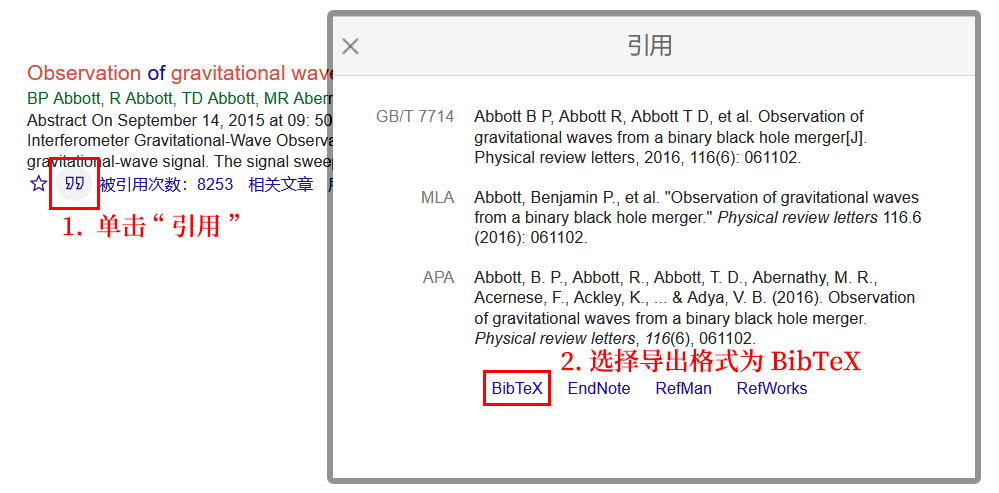
\includegraphics[width=10cm]{figure/AddBib.png}
                \label{fig:addbib}
            \end{figure}
        \item 在弹出框中,单击最下方\emph{Bibtex}的链接;
        \item 在弹出的网页中复制所有代码至\texttt{thesisbib.bib},并根据需要做一些改动;
        \item 在您的论文中使用\texttt{$\backslash$scite\{\}}引用相应的文献。
    \end{itemize}

    举个例子:在网页中将
    \begin{lstlisting}
@article{abbott2016observation,
    title={Observation of gravitational waves from a binary black hole    merger},
    author={Abbott, Benjamin P and Abbott, Richard and Abbott, TD and     Abernathy, MR and Acernese, Fausto and Ackley, Kendall and Adams,   Carl and Adams, Thomas and Addesso, Paolo and Adhikari, RX and    others},
    journal={Physical review letters},
    volume={116},
    number={6},
    pages={061102},
    year={2016},
    publisher={APS}
}
    \end{lstlisting}
    复制进\texttt{thesisbib.bib},在您的论文中使用\texttt{$\backslash$scite\{abbott2016observation\}}即可引用此文献。


    再来一个\scite{ashirov2008tetramerization} ,网络上的资源引用\scite{buctthesis},等。

	
\section{附录}\label{sec:app}
在\texttt{buctthesis.tex}中以
\begin{lstlisting}[firstnumber=68]
\appendix
\end{lstlisting}
命令作为附录部分的开始。与正文类似,只需往\texttt{chapter/app1.tex}等加入内容即可。除了编号使用大写字母之外都一样。见附录~\ref{app:1}。

\section{符号说明}\label{sec:deno}
	\emph{符号说明}部分的源文件位于\texttt{chapter/denotation.tex}。
    《规范》中未详细规定\emph{符号说明}的格式。这里附上一个以表格展示的代码:
    \begin{lstlisting}[caption=以表格展示的最小示例]
\begin{longtable}[c]{p{2.5cm}p{12cm}}
    \toprule
    \textbf{符号} & \textbf{说明} \\* \midrule
    \endfirsthead
    \multicolumn{2}{r}{\bfseries (接上表)} \\
    \toprule
    \textbf{符号} & \textbf{说明} \\* \midrule
    \endhead
    \bottomrule
    \endfoot
    \endlastfoot

    符号1   & 说明1     \\
    符号1   & 说明2     

    \\* \bottomrule
\end{longtable}        
    \end{lstlisting}

    本文档的\emph{符号说明}部分就是以此方式编辑,并展示了一个跨页表格的样式。详细代码请参见\texttt{denotation.tex}源代码和本手册\emph{符号说明}部分。

\section{致谢}
    \emph{致谢}部分的源文件\texttt{chapter/acknowledgement.tex},使用\texttt{acknowledgement}环境,往里面写入感谢的话就可以啦。
    \begin{lstlisting}
\begin{acknowledgement}
    % Words here.
    ...
\end{acknowledgement}
    \end{lstlisting}

\section{其他}\label{sec:other}

    \subsection{脚注}
    本模板采用数字脚注,跨章重置计数,使用命令\texttt{$\backslash$footnote}。前方高能\footnote{我是可爱的脚注}。

    \subsection{列表环境}
    本模板提供了三种列表环境:不编号的\texttt{itemize}、编号的\texttt{enumerate}和使用关键字的\texttt{description}环境。上面三种列表环境可以嵌套使用(至多四层),且会自动处理不同层次的缩进和编号:
    \begin{itemize}
        \item 一条
        \item 次条
        \item 这一条可以分为\dots
            \begin{itemize}
            \item 子一条
            \end{itemize}
        \end{itemize}
    稍复杂一点的,如:
        \begin{enumerate}
            \item 中文
            \begin{description}
                \item[文言文] 古代汉语
                \item[白话文] 现代汉语
                \begin{enumerate}
                    \item 口语
                        \begin{enumerate}
                            \item 普通话
                            \item 方言
                        \end{enumerate}
                    \item 书面语
                    \end{enumerate}
            \end{description}
            \item English
        \end{enumerate}
    \subsection{\texttt{hyperref}宏包的设置}
    这里不是论文要求所必须的,但是为了方便使用和查看还是做了设置,位于宏包文件\texttt{buctthesis.sty}的最后:
    \begin{lstlisting}[firstnumber=388]
\hypersetup{
    colorlinks=false,             % 不使用彩色文字链接
    linkcolor=black,
    bookmarksnumbered=true,       % 书签中,章节编号
    bookmarksopenlevel=\maxdimen, % 书签目录层次
    citecolor=green,              % 引用标记颜色
    pdfhighlight=/N,              % 点击链接时:/N外观不变;/P黑色半框;/O黑色边框
    breaklinks=true,              % 链接允许断行
}
    \end{lstlisting}
